Programowanie dynamiczne ma zastosowanie w problemach wykazujących 
własność \emph{optymalnej podstruktury} –
to znaczy, kiedy optymalne rozwiązanie problemu 
łatwo jest uzyskać znając optymalne rozwiązania podproblemów. 

\subsection{Znajdowanie najdłuższego podciągu rosnącego}
Rozważmy następujący problem: 
\begin{itemize}
	\item[] \textbf{Dane.} Pewien ciąg $c = c_1,c_2, \ldots, c_n$
	\item[] \textbf{Szukane.} Dowolny najdłuższy podciąg 
	$c_{i_1},c_{i_2},\ldots, c_{i_k}$ ciągu $c$, taki, że
	$i_1 < i_2 < \ldots < i_k$ oraz $c_{i_1} < c_{i_2} < \ldots < c_{i_k}$.    
\end{itemize}

Przykładowo, dla wejściowego ciągu $(3, 1, 8, 2, 5)$ odpowiedzią będzie
ciąg $(1, 8, 5)$.

W pierwszym kroku rozwiązywania problemów programowania dynamicznego szukamy
odpowiedniego podproblemu. Dla ułatwienia zareprezentujmy ciąg $c$ jako 
graf skierowany $G$, w którym wierzchołkami są elementy ciągu $c$ oraz 
istnieje krawędź z wierzchołka $c_i$ do wierzchołka $c_j$ jeśli $x < y$
oraz $i < j$. 
Opisany graf dla powyższego przykładu przedstawiony jest na rysunku
\ref{fig:example111_max_length}.

\begin{figure}[H]
	\centering
	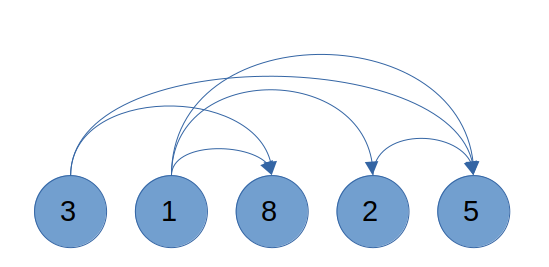
\includegraphics[width=0.4\textwidth]{data/prblm1_ex_graph.png}
	\caption{ }
	\label{fig:example111_max_length}
\end{figure}

Uprośćmy tymczasowo analizowany problem do problemu znajdowania 
długości najdłuższego rosnącego podciągu. Utwórzmy tablicę \textit{T} 
(numerujemy od 1), w której na indeksie $i$ 
będziemy przechowywać długość najdłuższego podciągu, dla którego $c_i$
jest jego ostatnim elementem. Przypuśćmy, że wypełniliśmy tablicę 
$T$ do ($i-1$)-szego elementu.
Wtedy, aby poznać wartość na $i$-tym indeksie, wystarczy przeanalizować 
wszystkie te wierzchołki w grafie $G$, które mają skierowaną krawędź na
$i$-ty wierzchołek.

\begin{figure}[H]
	\centering
	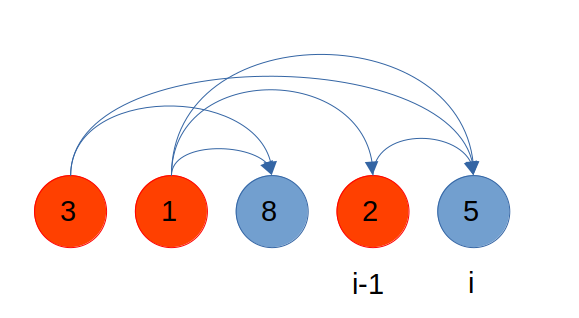
\includegraphics[width=0.4\textwidth]{data/prblm1_ex_graph2.png}
	\caption{  }
	\label{fig:example112_max_length}
\end{figure}

Niech $I$ będzie zbiorem indeksów wszystkich elementów ciągu $c$, które są 
mniejsze niż $c_i$, wtedy 
\[T[i]=\max\limits_{j \in I}\{T[j]\} + 1.\]

Jeśli wypełnimy całą tablicę $T$ według powyższej procedury, odpowiedzią
będzie maksymalny element tablicy $T$.

\begin{algorithm}[H]
	\caption{Znajdowanie najdłuższego rosnącego podciągu}\label{MaxIncreasingSubseqenceLength}
	\begin{algorithmic}[1]
		\Procedure{MaxIncreasingSubseqenceLength}{$c=(c_1,c_2, \ldots, c_n)$: ciąg}
		\State Utwórz tablicę $n$-elementową $T$
		\State Ustaw wartość każdej komórki tablicy $T$ na $1$
		\State $i \gets 2$
		\While{$i \leq n$}
		\State $j \gets 1$
		\While{$j \leq i - 1$}
		\If{$c_i \geq c_j$} 
		\State \textbf{continue}
		\EndIf
		\If{$T[i] \leq T[j] + 1$} 
		\State $T[j] \gets T[i]$
		\EndIf
		\EndWhile
		\EndWhile
		\State \Return $\max\limits_{1 \leq i \leq n}\{T[i]\}$
		\EndProcedure
	\end{algorithmic}
\end{algorithm}

Złożoność czasowa powyższego rozwiązania jest rzędu $n^2$. 

Powyższy algorytm można bardzo łatwo zmodyfikować w taki sposób, aby
możliwe było zwrócenie podciągu stanowiącego rozwiązanie (problem pierwotny).
Wystarczy utworzyć tablicę $P$, która na indeksie $i$
będzie zapisywać indeks ostatniego elementu, który spełnił 
warunek $T[i] \leq T[j] + 1$. Ustalmy, że $-1$ będzie oznaczało, że 
takiego elementu nie ma (tzn. $c_i$ jest pierwszym elementem podciągu).

\begin{algorithm}[H]
	\caption{Znajdowanie najdłuższego rosnącego podciągu.}\label{MaxIncreasingSubseqence}
	\begin{algorithmic}[1]
		\Procedure{MaxIncreasingSubseqence}{$c = (c_1,c_2, \ldots, c_n$): ciąg}
		\State Utwórz tablicę $n$-elementową $T$
		\State Ustaw wartość każdej komórki tablicy $T$ na $1$
		\State Utwórz tablicę $n$-elementową $P$
		\State Ustaw wartość każdej komórki tablicy $P$ na $-1$
		\State $i \gets 2$
		\While{$i \leq n$}
		\State $j \gets 1$
		\While{$j \leq i - 1$}
		\If{$c_i \geq c_j$ } 
		\textbf{continue}
		\EndIf
		\If{$T[i] \leq T[j] + 1$ } 
		\State $T[j] \gets T[i]$
		\State $P[i] \gets j$
		\EndIf
		\EndWhile
		\EndWhile
		\State $m = \max\limits_{1 \leq i \leq n}\{T[i]\}$ 
		\State Utwórz tablicę $m$-elementową $A$ reprezentującą
		kolejne wartości szukanego podciągu
		\State $i \gets m$
		\State $j \gets$ indeks elementu o wartości $m$
		\While{$i \geq 1$}
		\State $A[i] \gets c_j$
		\State $j \gets P[j]$
		\State $i \gets i - 1$
		\EndWhile
		\State \Return $A$
		\EndProcedure
	\end{algorithmic}
\end{algorithm}

\subsection{Problem wydawania reszty}
Rozważmy następujący problem:
\begin{itemize}
	\item[] \textbf{Dane.} Nominały monet $n_1$, $n_2$, 
	$\ldots$, $n_k \in \mathbb{N}$ oraz kwota $K \in \mathbb{N}$
	\item[] \textbf{Szukane.} Ciąg liczb naturalnych $a = a_1$, $a_2$,
	$\ldots$ $a_k$ taki, że 
	\[\sum\limits_{i=1}^{k} a_in_i = K \text{ oraz suma } 
	\sum\limits_{i=1}^{k} a_i
	\text{ jest najmniejsza możliwa,}\]
	innymi słowy: szukamy sposobu na wydanie kwoty $K$ z użyciem
	jak najmniejszej liczby monet.
\end{itemize}

Na początek zaobserwujmy, że jeśli $a = a_1$, $a_2$,
$\ldots$ $a_k$, to rozwiązanie optymalne powyższego problemu, to 
zmniejszenie $a_i \geq 1$ ($i \in [k]$) o $1$, powinno 
poskutkować powstaniem rozwiązania problemu dla kwoty $K - n_i$.
To stwierdzenie musi być prawdziwe, bo inaczej moglibyśmy
skonstruować rozwiązanie o mniejszej liczbie monet
niż optymalne, co jest sprzecznością.

Przykładowo, dla $K = 13$ i nominałów $(1, 2, 5)$, optymalnym
rozwiązaniem jest ciąg $(1, 1, 2)$. Wtedy ciąg $(0, 1, 2)$
jest optymalnym rozwiązaniem dla $K = 12$, ciąg 
$(1, 0, 2)$ jest optymalnym rozwiązaniem dla $K = 11$ oraz
ciąg $(1, 1, 1)$ jest optymalnym rozwiązaniem dla $K = 8$.

Z powyższego stwierdzenia wynika, że otrzymanie optymalnego 
rozwiązania dla kwoty $K$ jest możliwe po przeanalizowaniu 
\emph{wszystkich} optymalnych rozwiązań dla kwot $K - n_i$,
co oznacza że udało nam się znaleźć optymalną podstrukturę.

Tak samo jak w przypadku problemu znajdowania najdłuższego 
podciągu rosnącego, rozważmy uproszczoną wersję problemu, 
w której interesować nas będzie nie ciąg $a$, ale 
liczba monet w optymalnym rozwiązaniu. 

Zdefiniujmy tablicę $T$ (indeksowaną od $0$) jako 
tablicę rozmiaru $K + 1$, w której komórka $T[i]$ ($i \in {0, 1, \ldots, K}$)
przechowuje liczbę monet potrzebną do optymalnego wydania kwoty równej $i$.
Z powyższych rozważań
wiadomo, że jeśli tablica jest wypełniona do $(i-1)$-szego
elementu ($i \in {0, 1, \ldots, K}$) włącznie, to 
\begin{equation}
	T[i] = \min_{1 \leq j \leq k}\{T[i - n_j]\} + 1,
	\label{eq:min_change_making_relation}
\end{equation}
ponadto przy takiej definicji tablicy, możemy przyjąć, że $T[0] = 0$.

Na koniec zauważmy, że w badanym problemie
istnieją dane wejściowe, dla których nie 
istnieje rozwiązanie (w szczególności szukane rozwiązanie optymalne),
np. nie możemy wydać $K=3$ dla nominałów $(2, 4)$. 
Aby ułatwić zapis rozwiązania, jak i wykrywanie sytuacji, w których
ono nie istnieje, każda komórka tablicy $T$ będzie inicjowana
wartością $\infty$. Jeśli po wykonaniu się algorytmu zachodzi $T[K] = \infty$,
możemy zwrócić informację, że rozwiązanie nie istnieje.

\begin{algorithm}[H]
	\caption{Znajdowanie liczby monet optymalnego 
		rozwiązania w problemie wydawania reszty.}\label{MinCoinsCountChangeMaking}
	\begin{algorithmic}[1]
		\Procedure{MinCoinsCountChangeMaking}{$n_1,n_2, \ldots, n_k \in \mathbb{N}$: nominały monet, 
			$K \in \mathbb{N}$: kwota}
		\State Utwórz tablicę $(K+1)$-elementową $T$
		\State Ustaw wartość każdej komórki tablicy $T$ na $\infty$
		\State $T[0] = 0$
		\For{$i = 1, 2, \ldots K$}
		\For{$j = 1, 2, \ldots k$}
		\If{$i < n_j$} \textbf{continue}
		\EndIf
		\State $c = T[i - n_j] + 1$
		\If{$c < T[i]$} $T[i] \gets c + 1$
		\EndIf
		\EndFor
		\EndFor
		\If{$T[K] = \infty$} \textbf{return} \textit{null}
		\EndIf
		\State \textbf{return} \textit{T[K]}
		\EndProcedure
	\end{algorithmic}
\end{algorithm}

Powyższy algorytm ma złożoność pamięciową rzędu $K$ oraz czasową $K\cdot k$. 
Gdybyśmy chcieli ten sam problem rozwiązać rekurencyjną metodą, otrzymalibyśmy
złożoność czasową rzędu $2^K$ przez rozwiązywanie tych samych podproblemów kilkukrotnie.

Aby rozwiązać problem pierwotny, podobnie jak w znajdowaniu najdłuższego
podciągu rosnącego, utworzymy tablicę $P$ o długości $K+1$,
która będzie przechowywać w komórce o indeksie $i \in \{0, 1, \ldots K\}$, indeks $j$
nominału, takiego, że zależność \eqref{eq:min_change_making_relation}
będzie prawdziwa.

\begin{algorithm}[H]
	\caption{Znajdowanie liczby monet optymalnego 
		rozwiązania w problemie wydawania reszty}\label{ChangeMaking}
	\begin{algorithmic}[1]
		\Procedure{ChangeMaking}{$n_1,n_2, \ldots, n_k \in \mathbb{N}$: nominały monet, 
			$K \in \mathbb{N}$: kwota}
		\State Utwórz tablicę $(K+1)$-elementową $T$
		\State Ustaw wartość każdej komórki tablicy $T$ na $\infty$
		\State Utwórz tablicę $(K+1)$-elementową $P$
		\State $T[0] \gets 0$
		\For{$i = 1, 2, \ldots K$}
		\For{$j = 1, 2, \ldots k$}
		\If{$i < n_j$}  \textbf{continue}
		\EndIf
		\State $c = T[i - n_j] + 1$
		\If{$c < T[i]$} 
		\State $T[i] \gets c + 1$
		\State $P[i] \gets j$
		\EndIf
		\EndFor
		\EndFor
		\If{$T[K] = \infty$} \Return \textit{null}
		\EndIf
		
		\State Utwórz tablicę $T[K]$-elementową $A$ reprezentującą
		kolejne wartości ciągu.
		\State $i \gets K$
		\While{$i > 0$}
		\State $A[P[i]] \gets A[i] + 1$
		\State $i \gets i - n_{P[i]}$
		\EndWhile
		\State \textbf{return} A
		\EndProcedure
	\end{algorithmic}
\end{algorithm}

\subsection{Skreślanie ciągów}
% :((